% EBP course: session 9
% Thomas Klee
% 2019-03-27

% Preamble
\documentclass{beamer}
\usetheme{Singapore}
\usefonttheme[onlysmall]{structurebold}
\setbeamerfont{title}{shape=\itshape,family=\rmfamily}
\usepackage{graphicx}
\usepackage[english]{babel}
\usepackage[utf8x]{inputenc}
\usepackage{amsfonts, amsmath, amsthm, amssymb} % for math fonts, symbols and environments
\usepackage{xcolor}
\usepackage{booktabs}
\usepackage{ctable} % for command-driven tables
\usepackage{wasysym} 
%\hypersetup{colorlinks, allcolors = ., urlcolor = blue,} % to change color of URL from black to blue
\usepackage[natbibapa]{apacite}
\beamertemplatenavigationsymbolsempty % uncomment to add slide navigation symbols to each slide
\usepackage{appendixnumberbeamer}  % to suppress page numbers on extra slides
\setbeamertemplate{footline}[frame number] % to add slide numbers

% activate following line for custom appearance
% \usepackage{beamerthemesplit} 

\mode<presentation>

% information for title slide
\title{Diagnostic Accuracy, part 2 \\ \& Practice-Based Evidence}
\subtitle{}
\author{Evidence-Based Practice in Speech-Language Therapy \\ (SHSC 2033)}
\institute{Session 9}
\date{Thomas Klee \& Elizabeth Barrett}
\titlegraphic{
\includegraphics[width=6cm]{images/logo_CE_C.jpg}} % HKU logo

\begin{document}

% create title slide with information above
\begin{frame}
	\titlepage
\end{frame}

% 
\begin{frame}{Outline}
	\begin{enumerate}
	\item Diagnostic accuracy: post-test probability
	\item Practice-based evidence
	\item Evidence from client preferences
	\item Group discussion
	\end {enumerate}
\end{frame}

\section{Post-test probability}

% 
\begin{frame}
	\begin{center}
	\huge{Post-test Probability}
	\end{center}
\end{frame}

% 
\begin{frame}{Screening outcomes \footnote{\tiny{\citet{Klee2000}}}}
\begin{center}
\begin{tabular}{l | c | c | c}
\toprule
& Language & Language & \\
& delay & normal & Total \\ 
\hline
Screen $+$ & 10 & 2 & 12 \\
\hline
Screen $-$ & 1 & 51 & 52 \\
\hline
Total & 11 & 53 & 64 \\
\bottomrule
\end{tabular}
\end{center}
\end{frame}

% 
\begin{frame}{Classification accuracy measures \footnote{\tiny{Calculated using \emph{epiR} package of R \citep{RCoreTeam2019, Stevenson2017}}}} 
	\begin{center}
	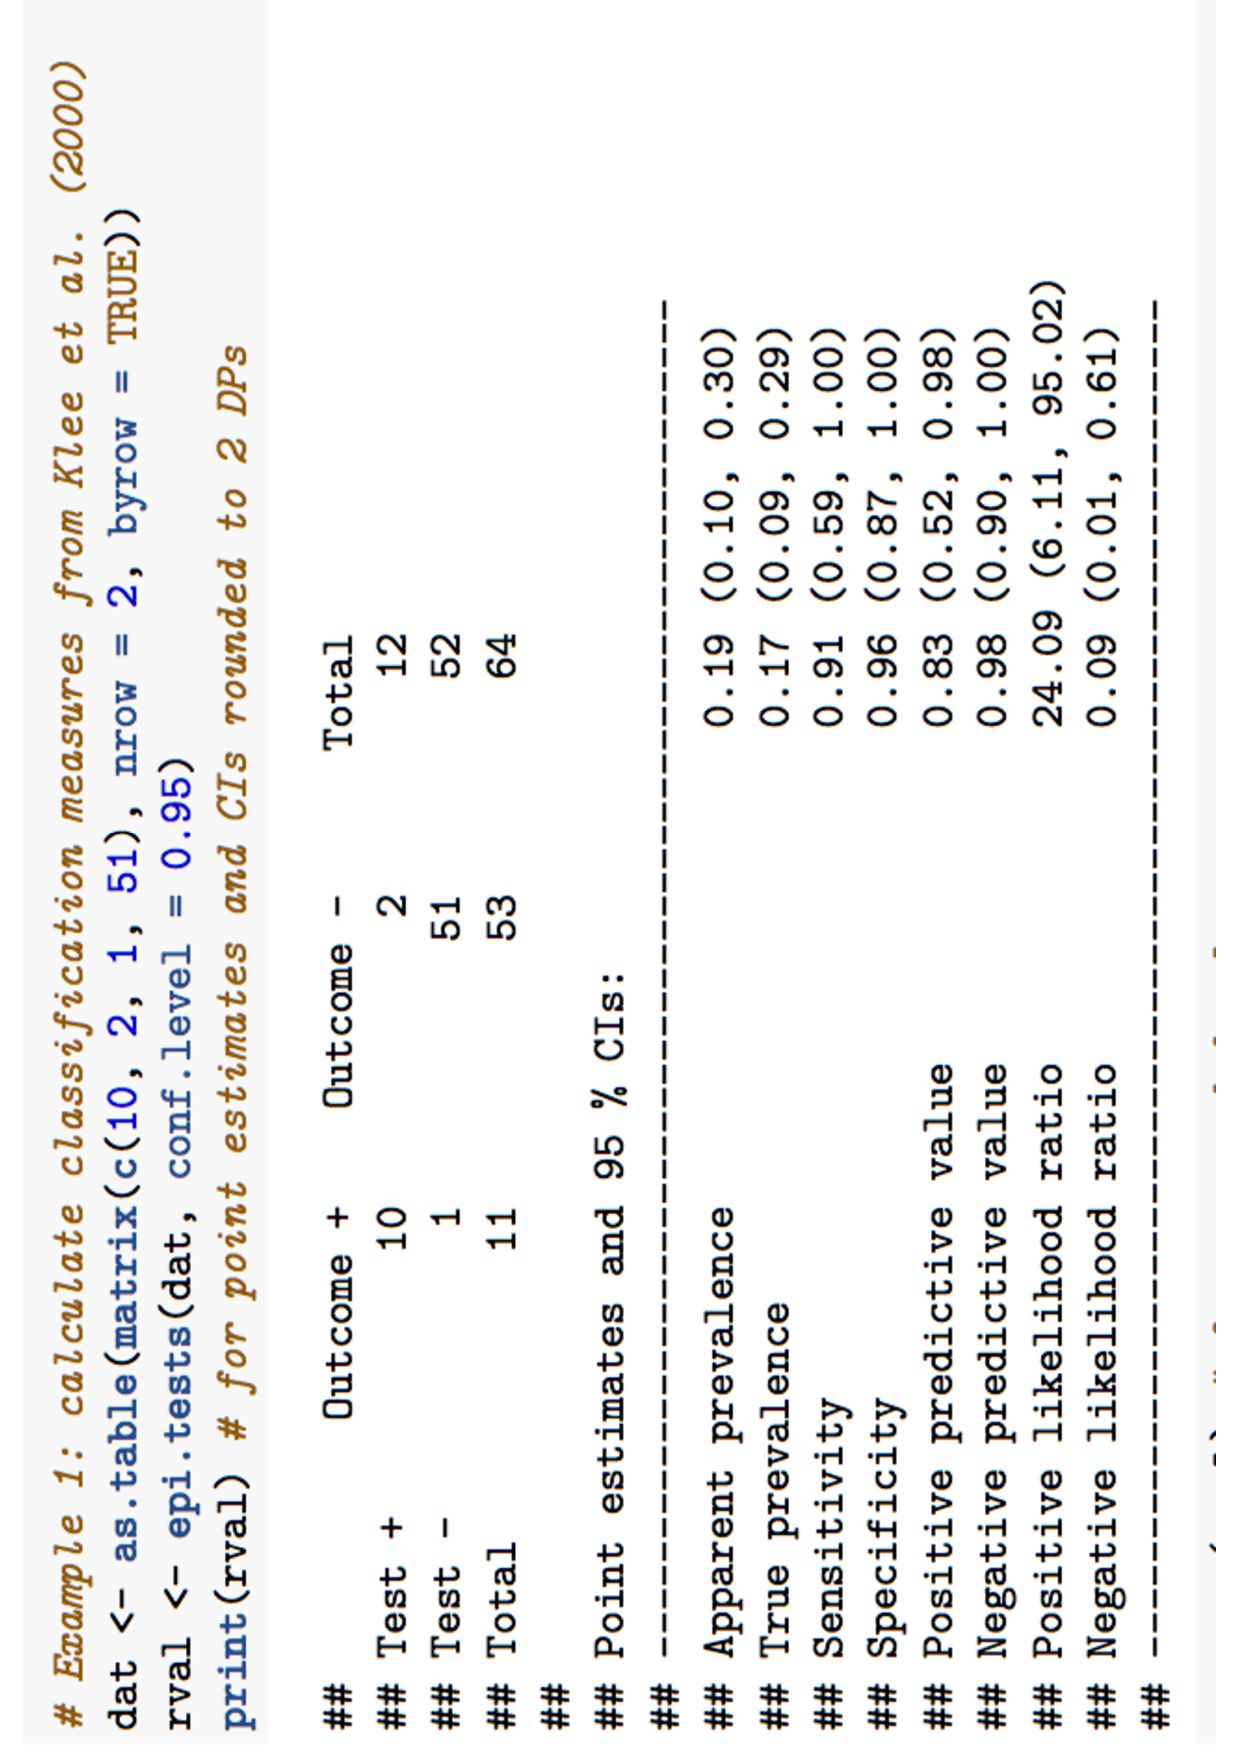
\includegraphics[angle=270, width=8cm]{images/epiR_screenshot1.pdf}
	\end{center}	
\end{frame}

\begin{frame}{What does \textbf{prevalence} refer to here?}
	\begin{itemize}
	\item \textbf{Apparent} prevalence: $12 / 64 = .19$ \footnote{Based on number of \textbf{test positives} in the sample.} 
	\item \textbf{True} prevalence: $11 / 64 = .17$ \footnote{Based on number of \textbf{cases} in the sample.}
	\item Do these accurately reflect population values?
	\end{itemize}
\end{frame}

% 
\begin{frame}{Be careful\dots}
	\begin{itemize}
	\item If the prevalence (base rate) of the disorder in the \alert{research sample} is different from the prevalence in the \alert{population}, the estimates reported for PPV and NPV will \alert{not} be accurate.
	\item Notice the results of our sample.
	\end{itemize}
\end{frame}

% 
\begin{frame}{Klee et al sample} 
	\begin{center}
	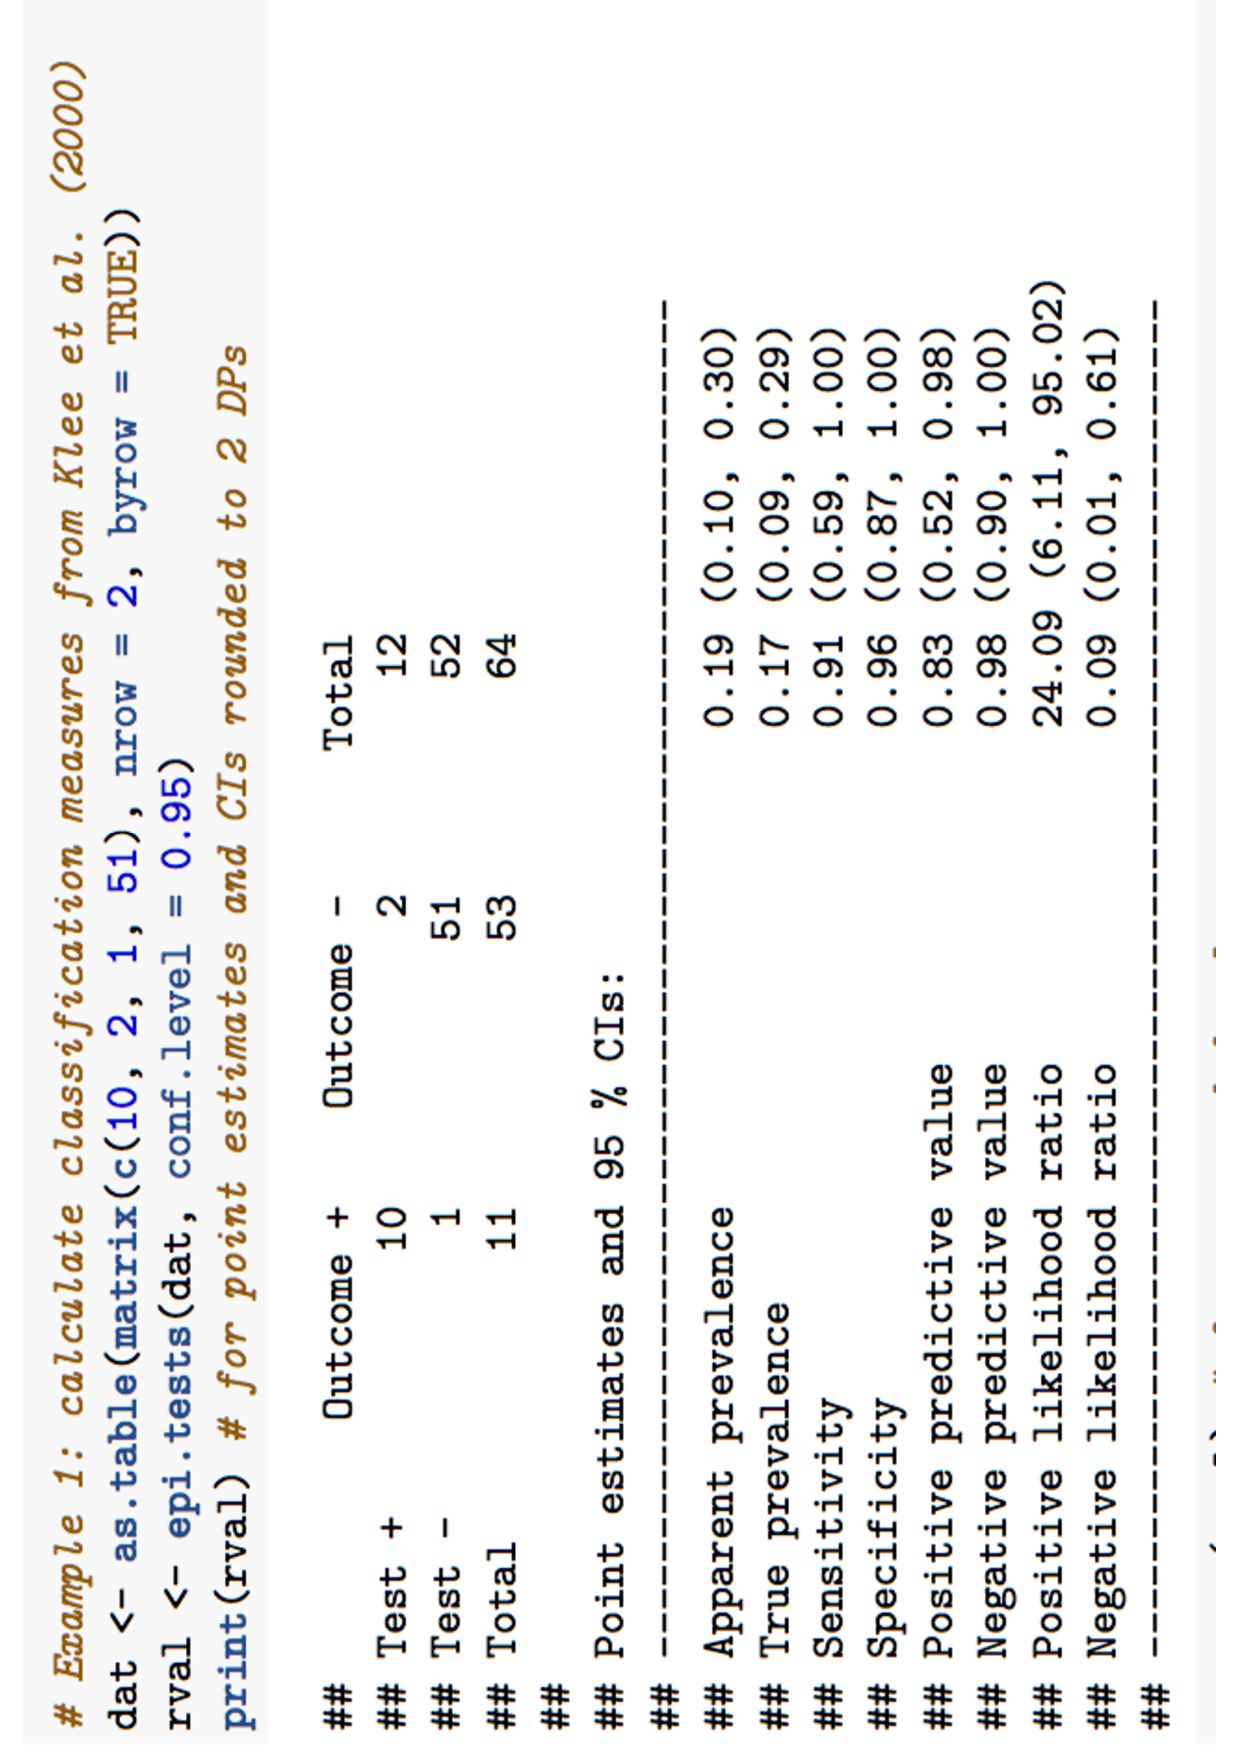
\includegraphics[angle=270, width=8cm]{images/epiR_screenshot1.pdf}
	\end{center}	
\end{frame}

% 
\begin{frame}{Summary}
	\begin{itemize}
	\item Sensitivity and specificity aren't affected by prevalence.
	\item Neither are the likelihood ratios, since they are based on sensitivity and specificity.
		\begin{itemize}
		\item LR+ $= Sensitivity / (1 - Specificity)$
		\item LR-- $= (1 - Sensitivity) /  Specificity$
		\end{itemize} 
	\item This is why LRs are preferable to PPV and NPV.
	\end{itemize}
\end{frame}

% 
\begin{frame}{LR+}
\begin{center}
\begin{tabular}{l | c | c }
\toprule
& Condition & Condition \\
& present & absent \\ 
\hline
Index test $+$ & \alert{True positive} & \alert{False positive} \\
\hline
Index test $-$ & False negative & True negative \\
\bottomrule
\end{tabular} \\
\end{center}

\begin{itemize}
	\item LR+ = Sensitivity / (1 - Specificity) 
	\item LR+ = proportion of TPs / proportion of FPs 
	\item LR+ = proportion of  (+) test results in those with the condition / proportion of (+) test results in those without the condition
\end{itemize}
\end{frame}

% 
\begin{frame}{Interpreting LRs \footnote{\tiny{\citet[p. 208]{Guyatt2008d}}}}
	\begin{itemize}
	\item LRs of  $>10$ or $<0.1$ indicate large and often conclusive changes from \textbf{pre- to post-test probability}.
	\item LRs of 5 to 10 and 0.1 to 0.2 indicate moderate shifts in \textbf{probability}.
	\item LRs of  2 to 5 and 0.2 to 0.5 indicate small (but sometimes important) shifts in \textbf{probability}.
	\item LRs of 1 to 2 and 0.5 to 1 alter \textbf{probability} to a small (and rarely important) degree.
	\end{itemize}
\end{frame}

% 
\begin{frame}{Post-test probability can be calculated if we know\dots}
	\begin{enumerate}
	\item the \alert{LR} associated with the test result
	\item the \alert{pre-test probability} of the condition \footnote{\tiny{taking the clinical setting and purpose into account (e.g., screening vs clinical assessment)}}
	\end{enumerate}
\end{frame}

% 
\begin{frame}{Basis of Bayes' theorem}
	\begin{center}
	We possess knowledge at any given point in time. \\
	$\downarrow$ \\ 
	We encounter new information (data).\footnote{\tiny{Based on our own experience, high quality research evidence, etc.}} \\
	$\downarrow$ \\ 
	We revise (update) our knowledge. 
	\end{center}
\end{frame}

% 
\begin{frame}{} 
	\begin{center}
	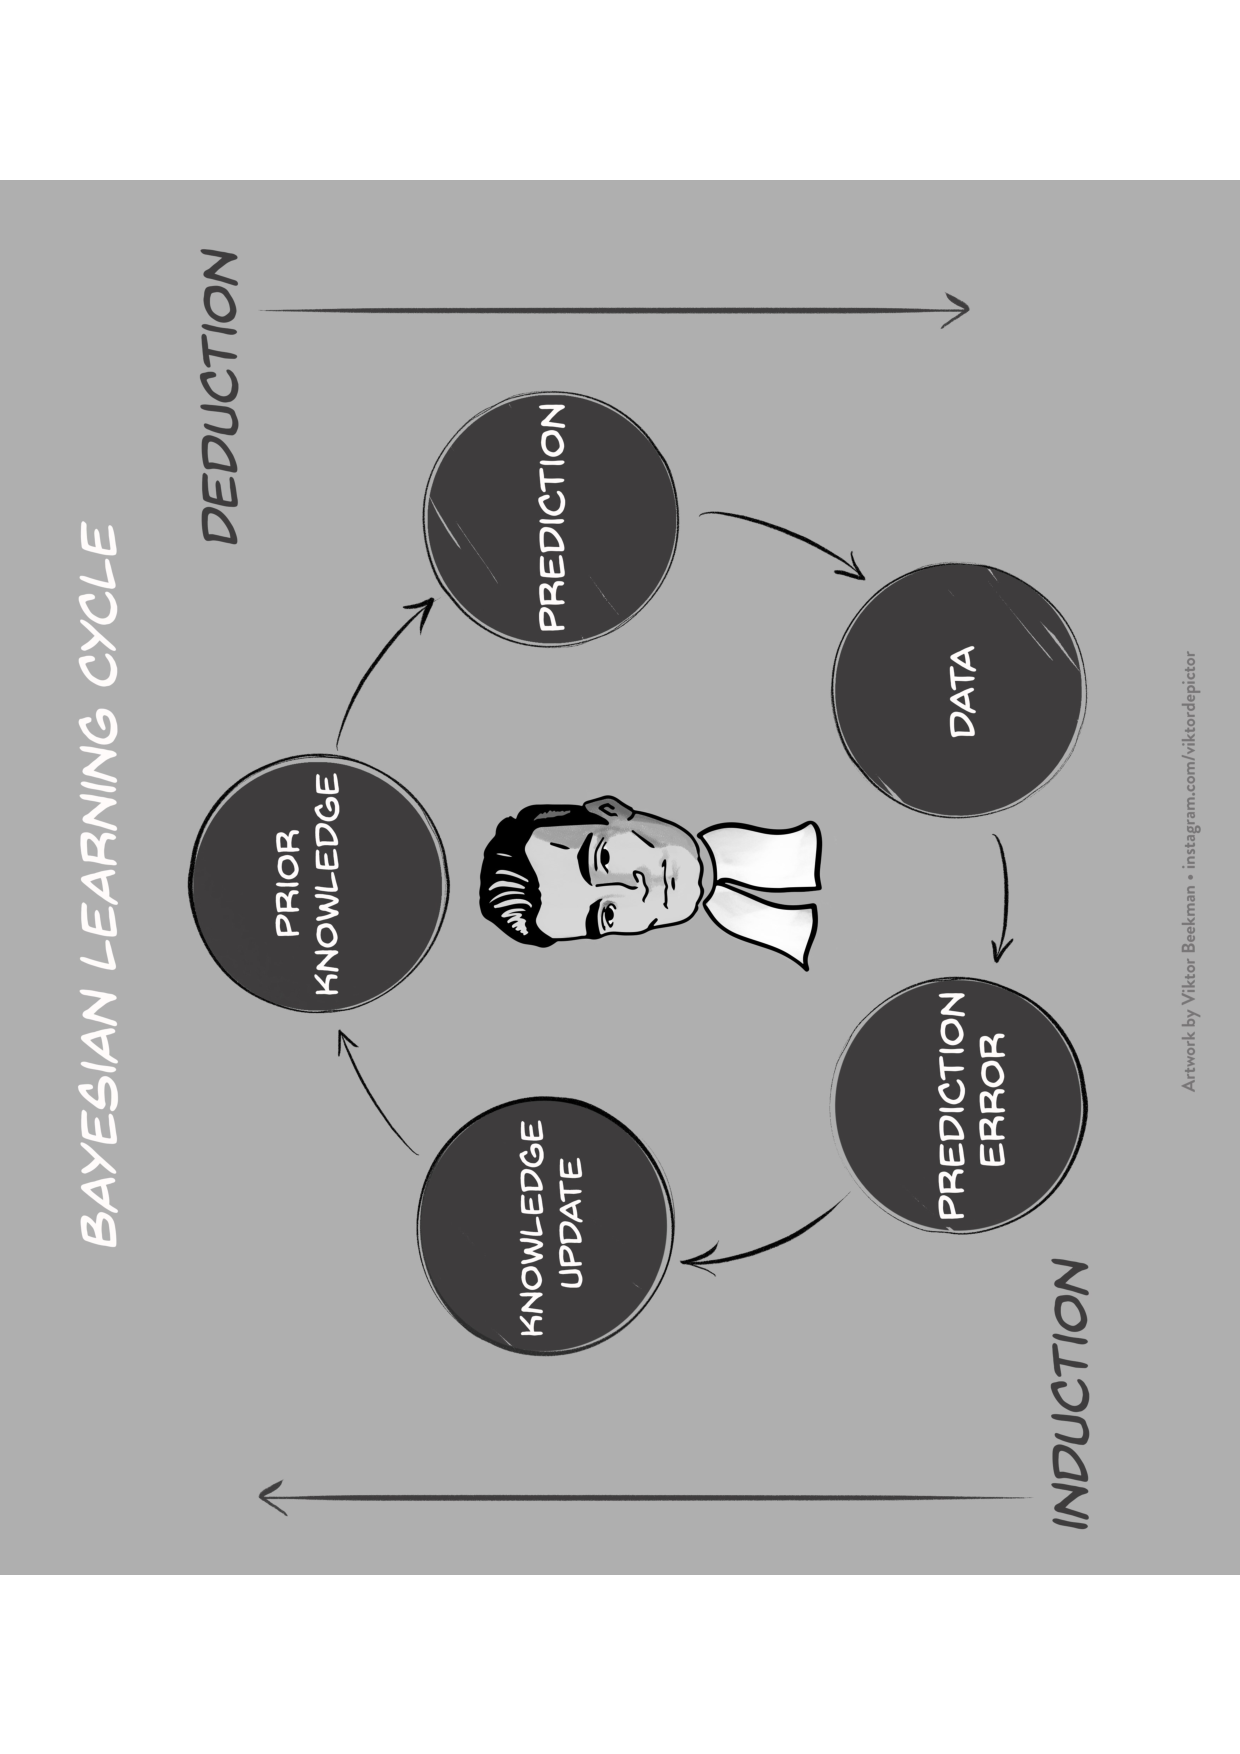
\includegraphics[angle=270, width=10cm]{images/BayesianLearningCycle.pdf}
	\end{center}	
\end{frame}

%
\begin{frame}{Bayes' theorem}
	\begin{quote} 
	``Bayes' theorem is concerned with conditional probability. That is, it tells us the probability that a theory or hypothesis is true \emph{if} some event has happened." \footnote{\tiny{\citet[p. 243]{Silver2012}}}
	\end{quote}
	
	\begin{quote}
	``\dots by updating our initial belief about something with objective new information, we get a new and improved belief." \footnote{\tiny{\citet[p. xi]{McGrayne2011}}}
	\end{quote}
\end{frame}

% 
\begin{frame}{Applying Bayesian thinking to clinical measures}
	\begin{center}
	We possess knowledge at any given point in time. \\
	 \alert{Prior (pre-test) probability} \\
	$\downarrow$ \\ 
	We encounter new information (data). \\
	 \alert{LR} \\
	$\downarrow$ \\ 
	We revise (update) our knowledge. \\
	 \alert{Posterior (post-test) probability} 
	\end{center}
\end{frame}

% 
\begin{frame}{LR Nomogram\footnote{\tiny{Estimate post-test probability with a ruler \citep[p. 285]{Haynes2006}}}}
	\begin{center}
	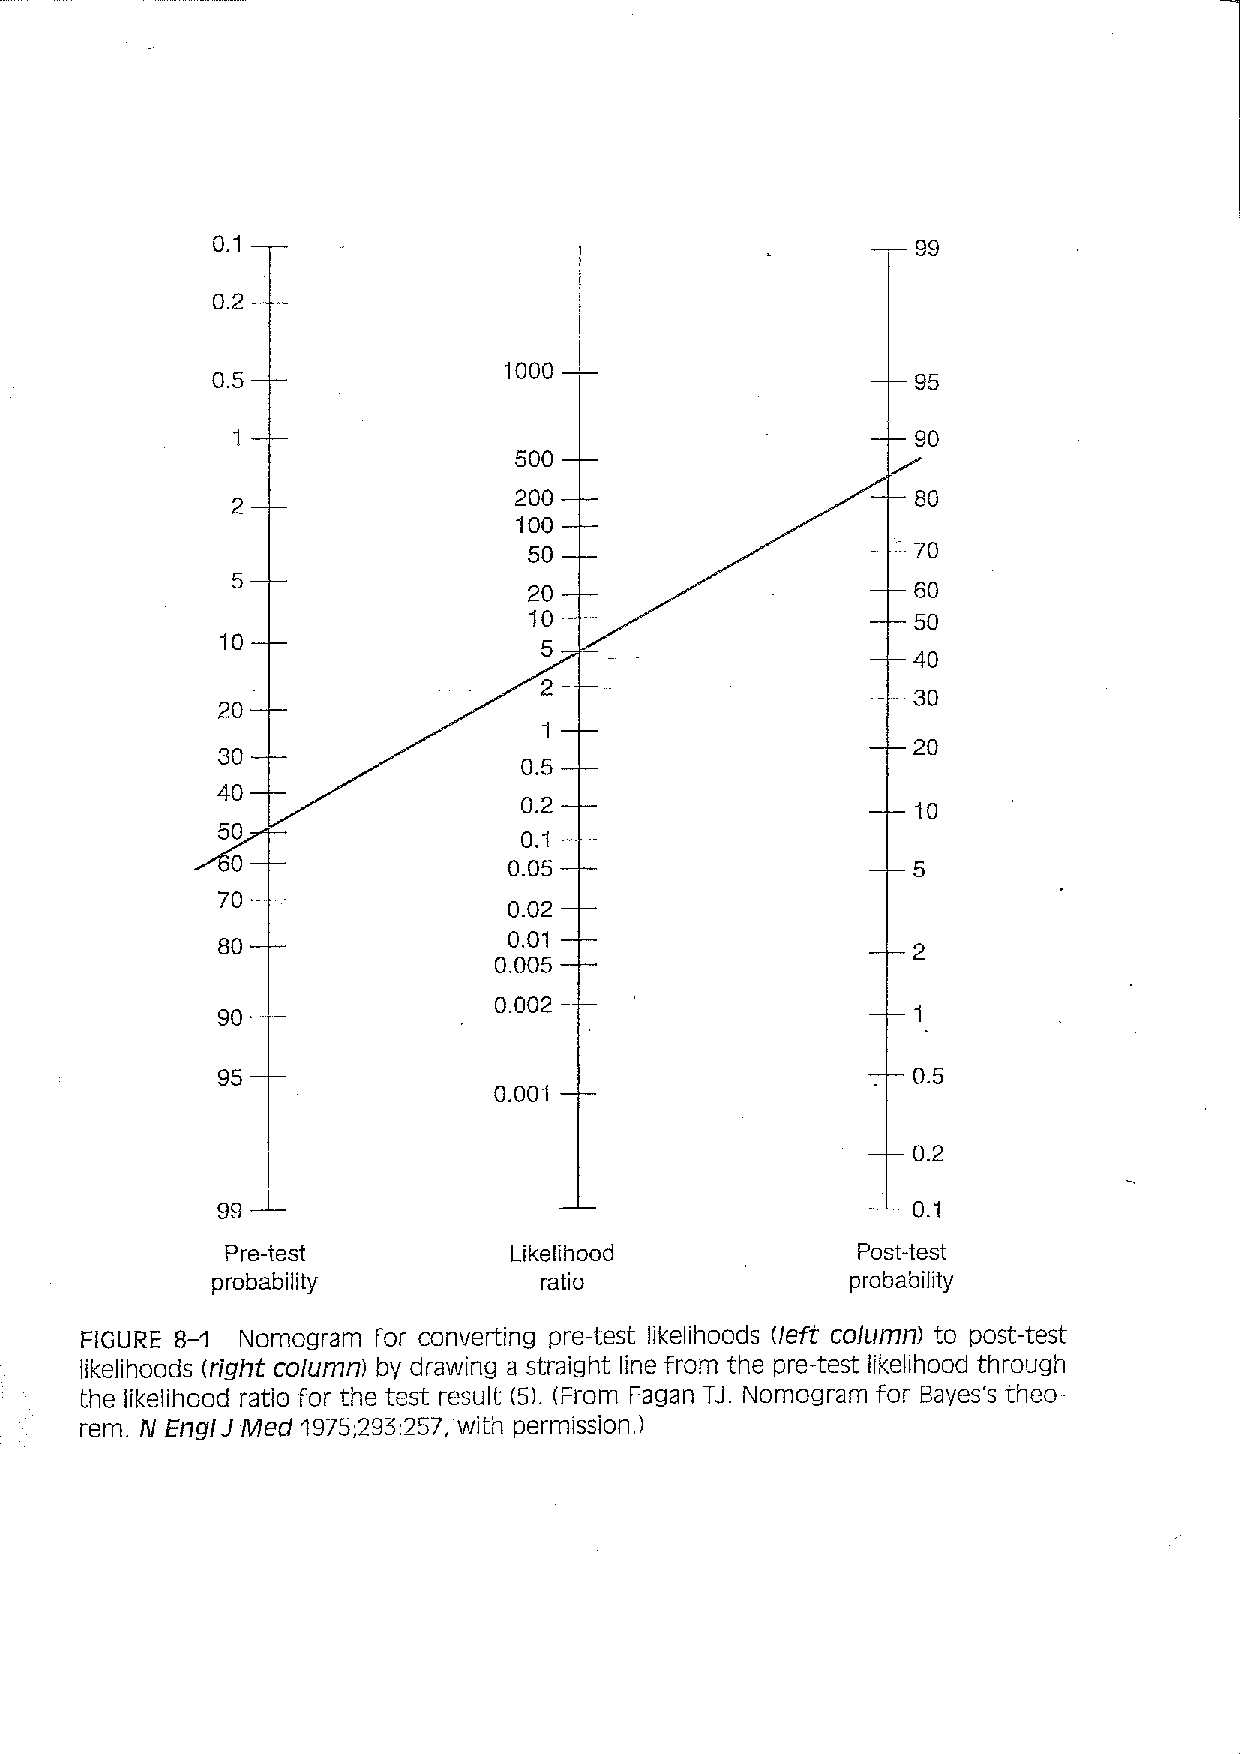
\includegraphics[height=7cm]{images/nomogram_haynes_2006.pdf}
	\end{center}	
\end{frame}

% 13 (not used, but same as following slide, with change of one word in last line, which I think is in error in epiR)
%\begin{frame}{Estimate it using R \footnote{\tiny{with \emph{epiR} package \citep{RCoreTeam2019, Stevenson2017}.}}}
%	\vspace{0.4cm}
%	Example: With a pre-test probability of 13\%, what's the post-test probability of having the condition, given the test result? \\
%
%	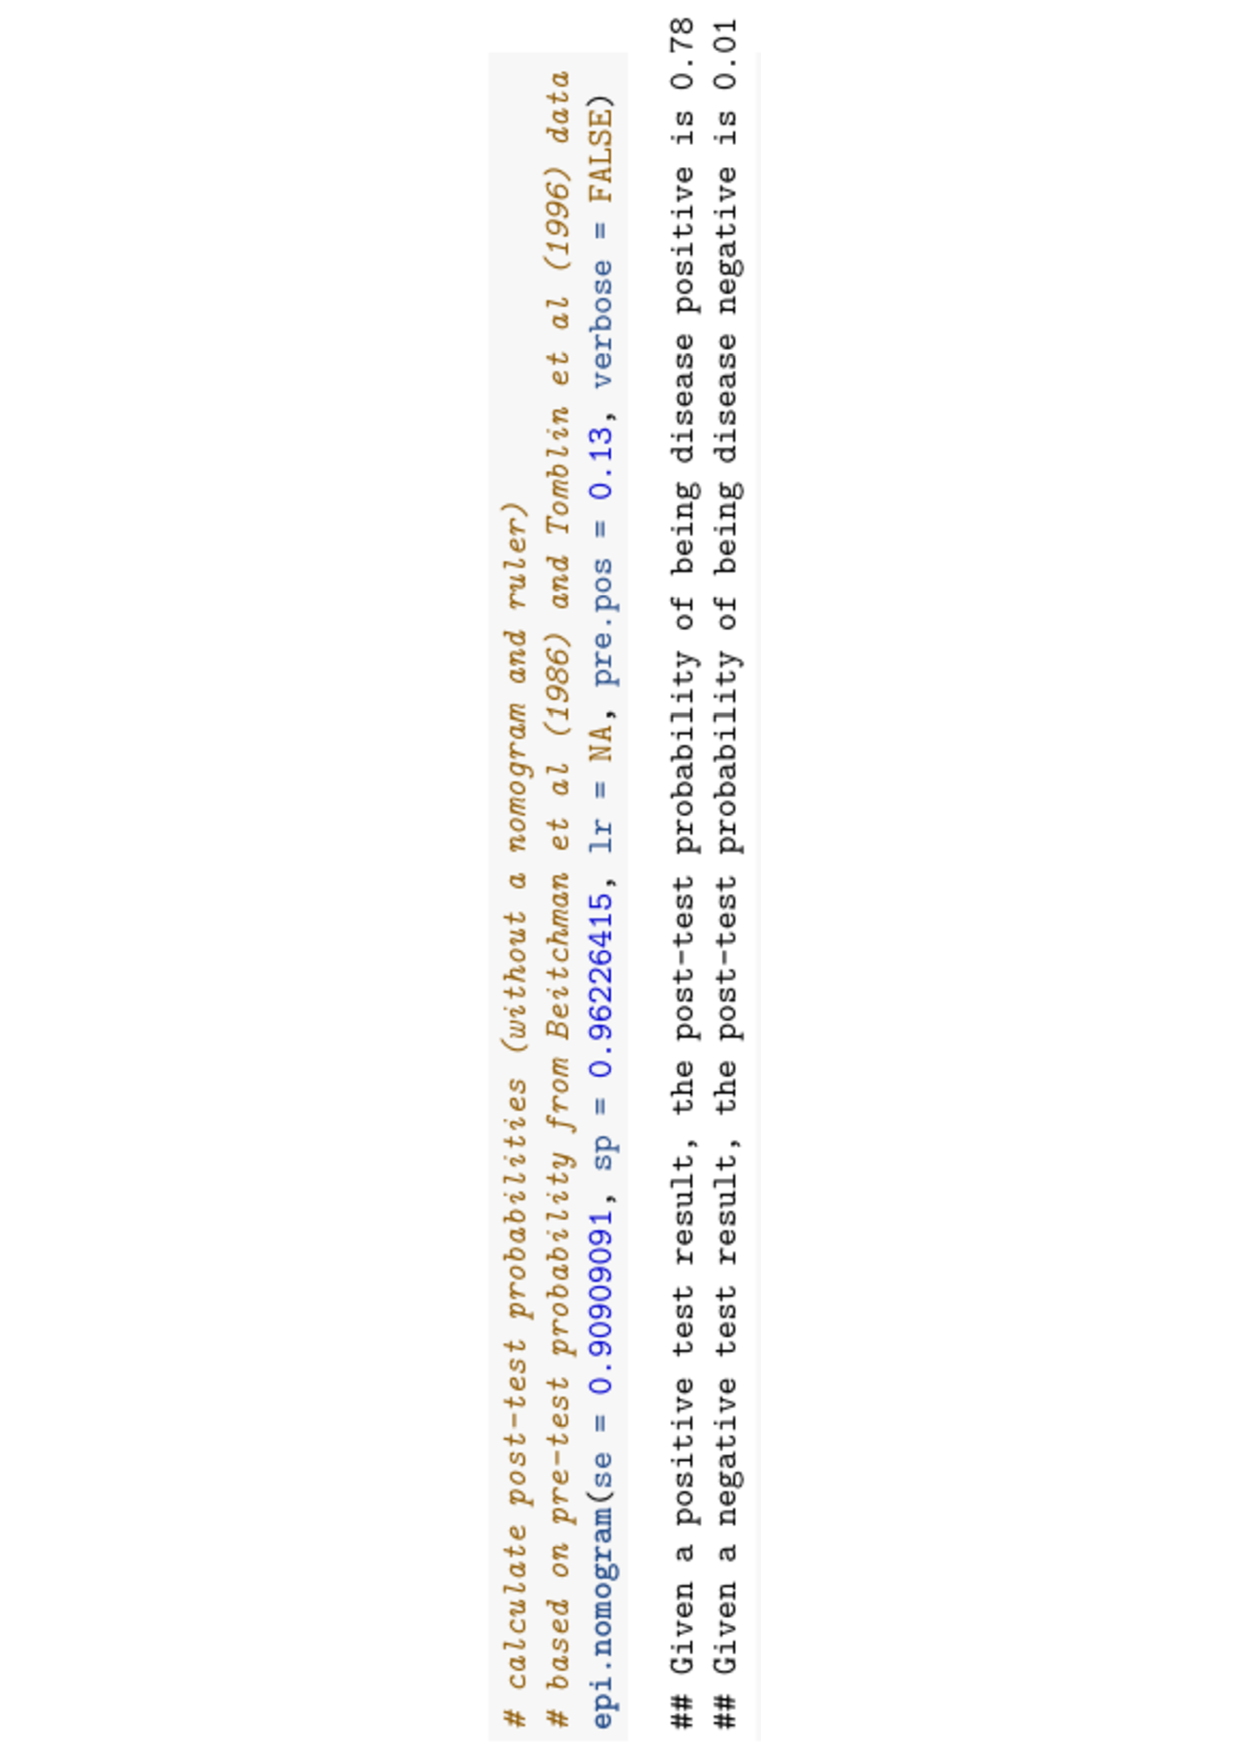
\includegraphics[angle=270, width=0.8\linewidth]{images/epiR_screenshot3.pdf}
%\end{frame}

% 
\begin{frame}{Estimate post-test probability with R \footnote{\tiny{with \emph{epiR} package \citep{RCoreTeam2019, Stevenson2017}.}}}
%	\vspace{0.4cm}
	\begin{itemize}
	\item Example: With a pre-test probability of 13\%,\footnote{\tiny{Based on prevalence data reported in Beitchman et al (1986) and Tomblin et al (1996)}} what's the post-test probability of having the condition, given the test result? \\
		\begin{itemize}
		\item[] \texttt{library(epiR)}
		\item[] \texttt{epi.nomogram(se = 0.90909091, sp = 0.96226415, \\ lr = NA, pre.pos = \alert{0.13}, verbose = FALSE)}
		\item[]
		\item[*] \texttt{Given a positive test result, the post-test probability of being disease positive is \alert{0.78}}
		\item[*] \texttt{Given a negative test result, the post-test probability of being disease negative\footnote{\tiny{I think this should read "disease positive".}} is \alert{0.01}}
		\end{itemize}
	\end{itemize}
\end{frame}

% 
\begin{frame}{Interpretation}
	\begin{itemize}
	\item Given a \alert{positive} screening result, there is a \alert{78\%} chance the child has the condition being screened for (language disorder).
	\item Given a \alert{negative} screening result, there is a \alert{1\%} chance the child has the condition.
	\item However, before concluding this, \textbf{notice which pre-test probability} these were based on.
		\begin{itemize}
		\item[$\rhd$] Adjust the pre-test probability if the sample prevalence differs from the population.
		\item[$\rhd$] Post-test probabilities are identical to PPV and NPV when the proportion of cases in the sample is the same as in the population.
		\end{itemize}
	\end{itemize}
\end{frame}

% 
\begin{frame}{What if this was a standardized test \\ given to a child referred for assessment? \footnote{\tiny{Hypothetical clinical population where half those referred for assessment are diagnosed with language disorder.}}}
	\begin{itemize}
	\item[] \texttt{library(epiR)}
	\item[] \texttt{epi.nomogram(se = 0.90909091, sp = 0.96226415, \\ lr = NA, pre.pos = \alert{0.50}, verbose = FALSE)}
	\item[]
	\item[*] \texttt{Given a positive test result, the post-test probability of being disease positive is \alert{0.96}} 
	\item[*] \texttt{Given a negative test result, the post-test probability of being disease negative\footnote{\tiny{I think this should read "disease positive".}} is \alert{0.09}} 
	\end{itemize}
\end{frame}

%
\begin{frame}{Estimate post-test probability with a leaf plot\footnote{\tiny{\citet{Coulthard2019}; data based on \citet{Klee2000}.}}}
	\begin{center}
		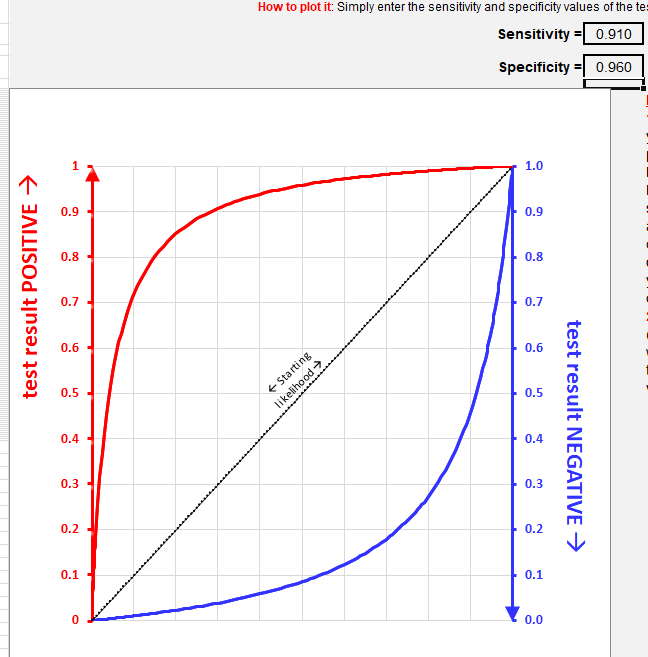
\includegraphics[width =6cm]{images/leafplot_kleedata.png}
	\end{center}
\end{frame}

%
\begin{frame}{Leaf plot for PSA results\footnote{\tiny{\citet{Coulthard2019}}}}
	\begin{center}
		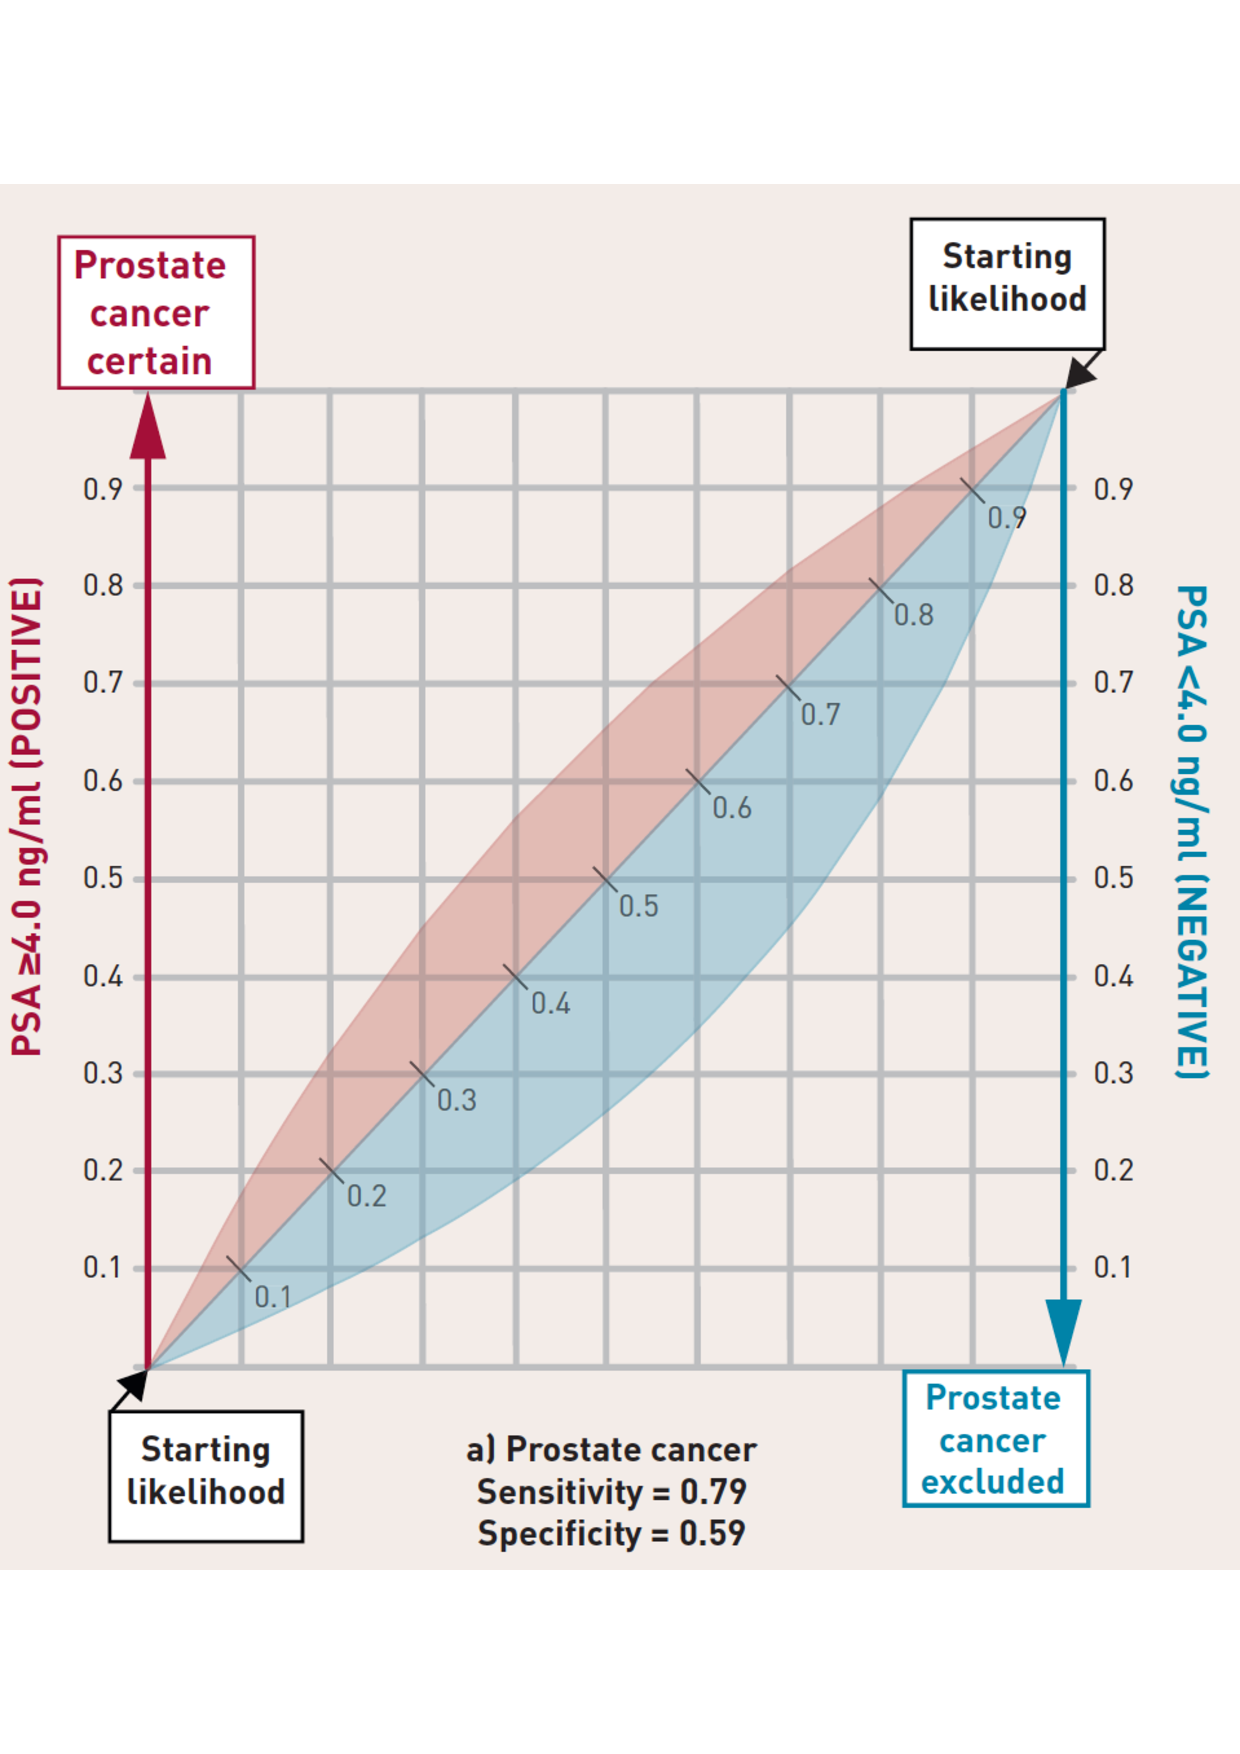
\includegraphics[width = 5cm]{images/leafplot_psa.pdf}
	\end{center}
\end{frame}

% 
\begin{frame}{Try it yourself with the person next to you}
\begin{itemize}
	\item Download leaf plot calculator from \url{https://childhealthafrica.org/downloads}. 
	\item Open it in MS Excel.
	\item Enter the sensitivity and specificity values from Klee et al. (2000) study.
	\item Explore how different pre-test probabilities affect post-test probability.
	\item Discuss how varying these numbers affects how you interpret test results.  
\end{itemize}
\end{frame}

% 
\begin{frame}{Estimate post-test probability with DocNomo}
	\begin{center}
		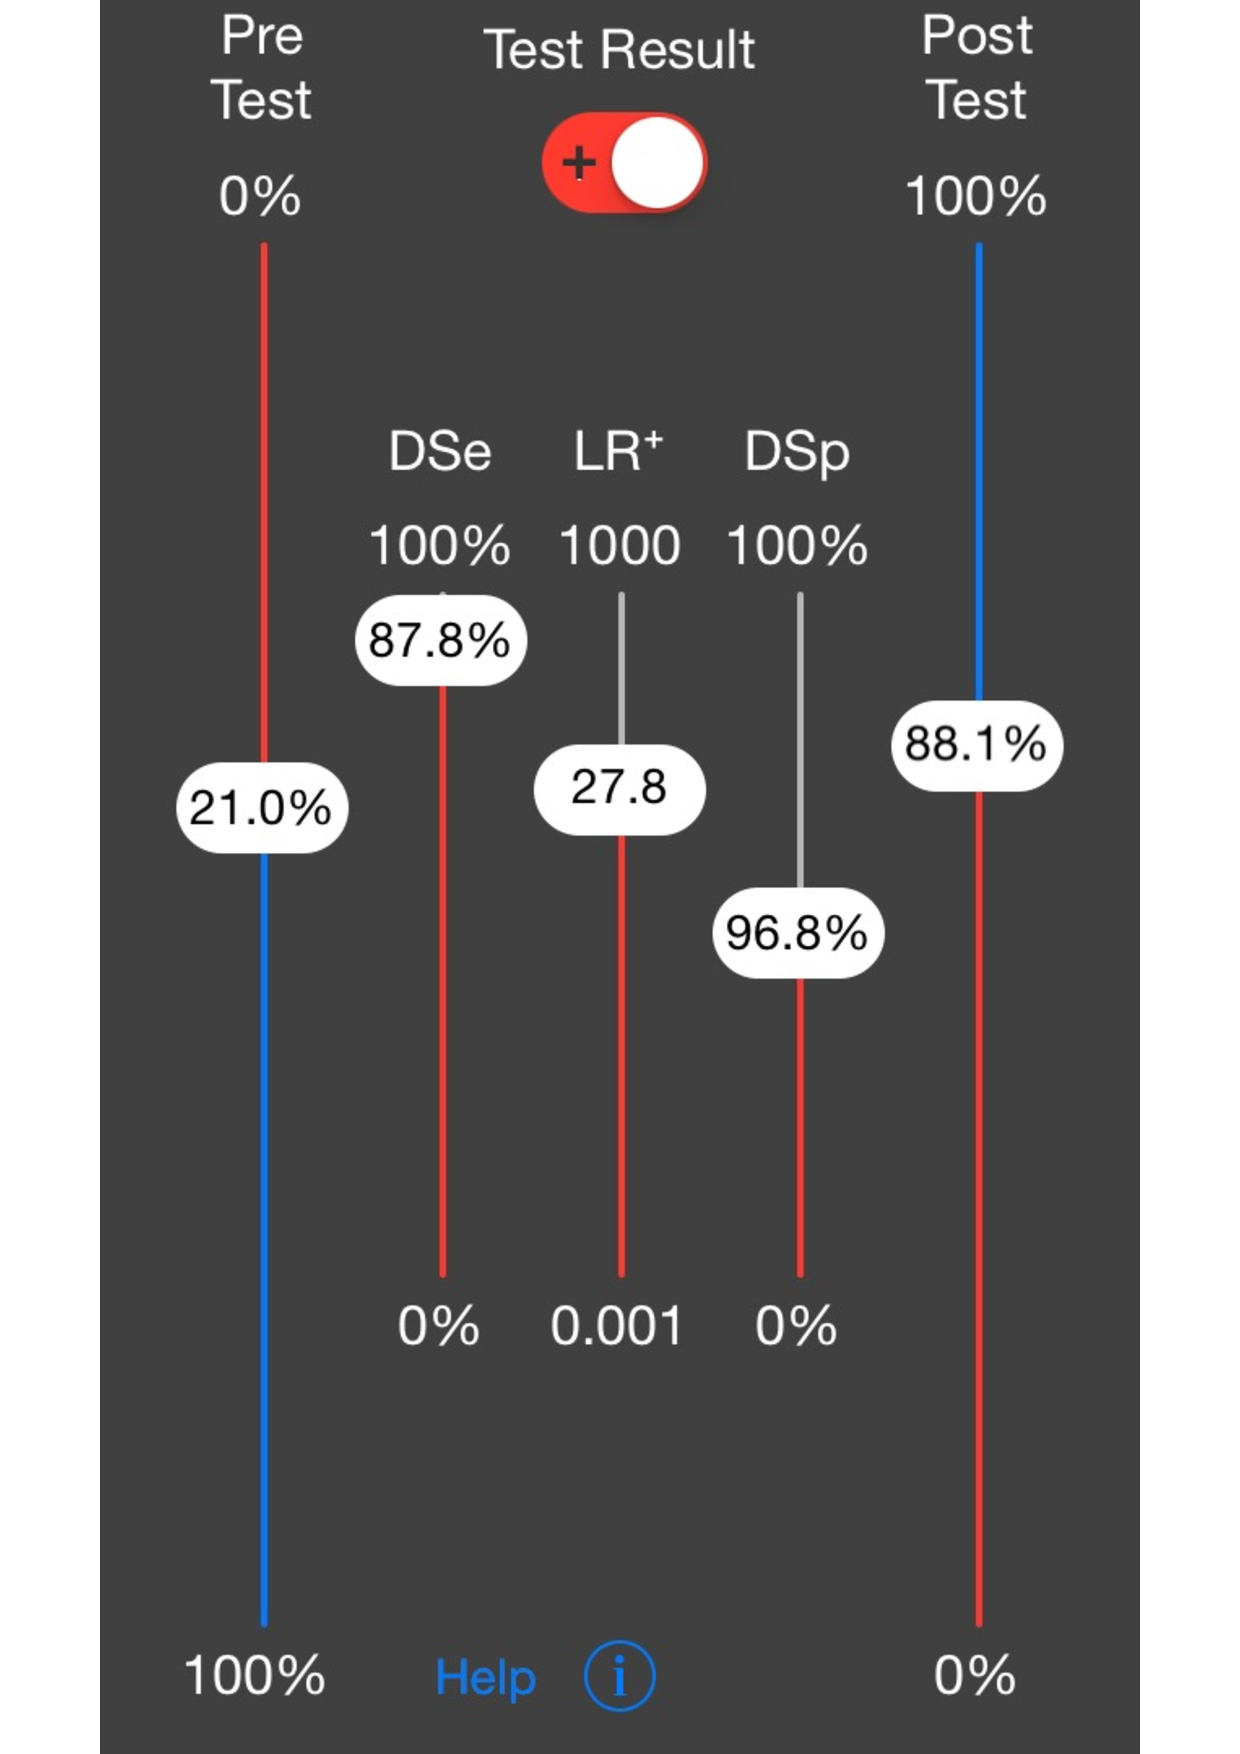
\includegraphics[height=6cm]{images/nomogram-app.pdf} \\
		\vspace{0.5cm}
		\texttt (Free for iOS devices. Values displayed are from another study.)
	\end{center}
\end{frame}

% the following 3 slides were used previously but not this time

% 
%\begin{frame}{Discuss with the person next to you}
%\begin{itemize}
%	\item In which phase of Sackett and Haynes' framework would you put the Klee et al. (2000) study?
%	\item[] (See following two slides for a reminder of their framework.)
%\end{itemize}
%\end{frame}

% 
%\begin{frame}{Framework for diagnostic research \footnote{\tiny{\citet{Sackett2002a}}}}
%	\begin{block}{Phase I}
%		\begin{itemize}
%		\item[-] Do those with the target disorder have different test results than those without the disorder? 
%		\item[-] Data generated under \alert{ideal} conditions rather than typical clinical settings
%		\item[-] Results at the group level
%		\end{itemize}
%	\end{block}
	
%	\begin{block}{Phase II}
%		\begin{itemize}
%		\item[-] Are those with certain test results more likely to have the target disorder than those with other test results? 
%		\item[-] Data from Phase I study can be used, but sensitivity and specificity are calculated
%		\item[-] Results at the individual level
%		\end{itemize}
%	\end{block}
%\end{frame}

% 
%\begin{frame}{Framework for diagnostic research}
%	\begin{block}{Phase III}
%		\begin{itemize}
%		\item[-] Does the test distinguish those with and without the target disorder among those in whom it is clinically reasonable to suspect that the disorder is present?
%		\item[-] Only done if results from Phase I--II studies are promising.
%		\item[-] Conducted in \alert{typical} clinical settings or conditions.
%		\item[-] Results at the individual level
%		\end{itemize}
%	\end{block}
	
%	\begin{block}{Phase IV}
%		\begin{itemize}
%		\item[-] Do those who undergo the diagnostic test fare better (in their ultimate health outcomes) than similar people who are not tested?
%		\item[-] Individuals must be randomised into groups.
%		\end{itemize}
%	\end{block}
%\end{frame}

\section{Practice-Based Evidence}

\begin{frame}
	\begin{center}
	\huge{Practice-Based Evidence}
	\end{center}
\end{frame}

% 
\begin{frame}{E$^3$BP}
	\begin{quote}
	``\dots the conscientious, explicit, and judicious integration of  best available\\
		\begin{enumerate}
		\item external \alert{evidence} from systematic research,
		\item \alert{evidence} internal to clinical practice, and
		\item \alert{evidence} concerning the preferences of a fully informed patient."  \footnote{\tiny{\citet[p. 2]{Dollaghan2007a}}}
		\end{enumerate}
	\end{quote}
\end{frame}

% 
\begin{frame}{Practice/patient-based evidence}
	\begin{quote}
	``The applicability of the external evidence from even a very strong study to an individual patient will need to be \alert{tested} rather than \alert{assumed}." \footnote{\tiny{\citet[p. 115]{Dollaghan2007a}}}
	\end{quote}
\end{frame}

\begin{frame}{Practice/patient-based evidence}
	\begin{itemize}
	\item How effective is this intervention with this client?
	\item Involves evaluating effectiveness of intervention \alert{with your own clients}
	\item CAPE: Checklist for Appraising Patient/Practice Evidence 
	\item ``Not\dots a critical appraisal form but rather a checklist of issues to consider in seeking valid, important evidence from clinical practice." \footnote{\tiny{\citet[p. 115]{Dollaghan2007a}}}
	\end{itemize}
\end{frame}

% 
\begin{frame}{CAPE: foreground question}
	\begin{description}
	\item[P] For \alert{your client or patient}
	\item[I] is \alert{the intervention}
	\item[O] associated with \alert{the outcome you've identified}
	\item[C] compared with \alert{contrasting intervention condition}?
	\end{description} 
\end{frame}

% 
\begin{frame}{CAPE: validity of the evidence \footnote{\tiny{\citet[p. 116]{Dollaghan2007a}}}}
	\begin{enumerate}
	\item Observational (A-B) or Experimental (e.g., A-B-A, alternating treatments, multiple baseline)?
	\item Randomization (e.g., targets to conditions, order of conditions)?
	\item Stable baseline(s)?
	\item Adequate length of treatment phase(s)?
	\item Treatment consistency, fidelity?
	\item Potential nuisance factor(s)?
	\item Valid and reliable measures?
	\item Measures administered with blinding?
	\end{enumerate}
\end{frame}

% 
\begin{frame}{CAPE: importance of the evidence \footnote{\tiny{\citet[p. 116]{Dollaghan2007a}}}}
	\begin{enumerate}
	\item Magnitude of treatment effect?
	\item Evidence of maintenance, generalization, and social validity of treatment effect?
	\item Substantial cost-benefit advantage?
	\end{enumerate}
\end{frame}

\section{Client Preferences}

% 
\begin{frame}
	\begin{center}
	\huge{Client Preferences}
	\end{center}
\end{frame}

% 
\begin{frame}{Client preferences}
	\begin{itemize}
	\item Concerns ``the preferences of fully informed patients relating to the clinical options they face" \footnote{\tiny{\citet[p. 123]{Dollaghan2007a}}}
	\item Client-centered care
	\item Qualitative research can inform this area of clinical practice.
	\item Establish a common ground with your client.
	\item Prepare information on clinical options.
	\item CAPP: Checklist for Appraising Patient Preferences
	\end{itemize}
\end{frame}

% 
\begin{frame}{CAPP: foreground question \footnote{\tiny{\citet[p. 128]{Dollaghan2007a}}}}
	\begin{description}
	\item[P] For \alert{this client, once fully informed of costs, risks, benefits}
	\item[I] is \alert{one clinical option}
	\item[O] a preferred \alert{outcome}
	\item[C] compared with \alert{other clinical options}?
	\end{description} 
\end{frame}

\section{Resources}

% 
\begin{frame}{Useful resources\footnote{\tiny{URLs checked on 2019-03-25}}}
	\begin{block}{Checklists for clinicians \citep{Dollaghan2007a}}
	CAPE to appraise patient/practice evidence (p. 159)\\
	CAPP to appraise evidence on patient preferences (p. 161)
	\end{block}

	\begin{block}{Description of diagnostic accuracy measures}
	\footnotesize{\url{http://www.students4bestevidence.net/ebm-for-diagnostic-tests/}}
	\end{block}

	\begin{block}{Estimating post-test probability}
		\begin{itemize}
		\item \url{https://ebm-tools.knowledgetranslation.net/calculator/diagnostic/} 
		\item \url{http://www.cebm.net/catmaker-ebm-calculators/} 
		\item \url{https://itunes.apple.com/us/app/docnomo/id901279945?mt=8}
		\item \emph{R} software's \emph{epiR} package \citep{Stevenson2017} 
		\end{itemize}
	\end{block}
\end{frame}

\section{Discussion}

% 
\begin{frame}{Group discussion}
	\begin{itemize}
	\item Break up into your assigned groups and discuss:
		\begin{enumerate}
		\item how you could begin to collect practice-based evidence with your own clients;
		\item how you could use CAPP with your own clients.
		\end{enumerate}
	\end{itemize}
\end{frame}

%\section*{References}

\begin{frame}[allowframebreaks] %[shrink=15] % to reduce font size of references
	\begin{center}
	\frametitle{References}
	\bibliographystyle{apacite}
	\small\bibliography{/Users/thomasklee/Documents/Bibtex/library}
	\end{center}
\end{frame}

% not used
%\begin{frame}{Classification accuracy measures \footnote{\tiny{Calculated using \emph{epiR} \citep{Stevenson2017}}}}
%\begin{center}
%\begin{tabular}{l  r  r}
%\toprule
%& Point estimates & 95\% CIs \\
%\midrule
%Apparent prevalence & 0.19 & (0.10, 0.30) \\
%\alert{True prevalence} & \alert{0.17} & (0.09, 0.29) \\
%Sensitivity & 0.91 & (0.59, 1.00) \\
%Specificity & 0.96 & (0.87, 1.00) \\
%Positive predictive value & 0.83 & (0.52, 0.98) \\
%Negative predictive value & 0.98 & (0.90, 1.00) \\
%Positive likelihood ratio & 24.09 & (6.11, 95.02) \\
%Negative likelihood ratio & 0.09 & (0.01, 0.61) \\
%\bottomrule
%\end{tabular}
%\end{center}
%\end{frame}

% calculate post-test probability of positive and negative screens without a nomogram and ruler

% not used
%\begin{frame}{Another way to estimate it \footnote{\tiny{Calculated using \emph{epiR} \citep{Stevenson2017}}}}
%	\begin{itemize}
%	\item[] \texttt{library(epiR)}
%	\item[] \texttt{epi.nomogram(se = 0.90909091, sp = 0.96226415, \\ lr = NA, pre.pos = 0.17, verbose = FALSE)} \\
%	\item[] 
%	\item[] The post-test probability of being disease positive is 0.83 
%	\item[] The post-test probability of being disease negative is 0.02
%	\end{itemize}
%\end{frame}

\end{document}%%